\chapter{Conclusiones y trabajos futuros}
\label{cap:conclusiones}

Una vez presentados los detalles del algoritmo desarrollado, su validación y verificación, en este último capítulo se exponen las conclusiones y se hace autocrítica del trabajo. Para finalizar, se proponen una serie de mejoras y ampliaciones que mejoren el comportamiento del algoritmo.

\section{Conclusiones}
\label{sec:conclusiones}

En este proyecto se ha desarrollado un algoritmo para hacer un seguimiento de los objetos más importantes del entorno de un robot. Como se ha explicado en capítulos anteriores, es muy importante filtrar la información recibida por parte de los sensores. En el caso de la cámara, la información se filtra dos veces. Una primera vez para detectar el objeto en cuestión en la imagen y otra para filtrar esa información y, en la medida de lo posible, reducir al máximo el ruido existente en las observaciones. De esta manera se consiguen resultados más precisos y robustos, lo que hace que el robot tome mejores decisiones. \\

Como conclusión general del proyecto se puede decir que se han cumplido satisfactoriamente los requisitos y objetivos marcados en el capítulo \ref{cap:objetivos}. El estado de las instancias del algoritmo está formado por la posición y la velocidad del objeto. Aunque la velocidad no es directamente medible, ésta se obtiene por inferencia a partir de las posiciones previas, obteniendo una medida bastante acertada. La colección de filtros es dinámica. Puede seguir varios objetos al mismo tiempo y, aunque sean indistinguibles para el detector, el algoritmo es capaz de emparejar las observaciones con su filtro correspondiente. El algoritmo se ejecuta en tiempo real y no consume muchos recursos. \\

La datos de entrada del algoritmo no están ligados a ningún sensor o detector concreto. El único imprescindible para ejecutarlo es la posición de un objeto en un instante determinado del tiempo. Igualmente tampoco influye en el funcionamiento del algoritmo si los objetos son dinámicos o estáticos. Si el comportamiento de estos está bien modelado, tendremos unos resultados precisos. \\

La implementación del algoritmo es independiente de la plataforma, es decir, en el código del núcleo de ésteno hay ninguna referencia a componentes dependientes del sistema donde se ha desplegado. Esto facilita enormemente su exportación y podría, incluso, compilarse como una biblioteca independiente y ser usado en cualquier proyecto. Se ha intentado diseñar el algoritmo de forma que sea flexible y fácilmente extensible, ya que cada situación se resuelve de una manera distinta. Por último, la precisión y robustez de los algoritmos de las observaciones se ha mejorado. Los datos son más fiables y estables que si se operase con ellos directamente desde el detector. \\

El desarrollo del proyecto se ha llevado a cabo mediante pequeñas iteraciones en las que se han ido implementando cada una de las partes del algoritmo. Se ha puesto especial énfasis en la programación de las operaciones matemáticas. Muchas de las ecuaciones son bastante largas y complejas, hecho que provoca muchos pequeños fallos a la hora de escribir el código. Un simple cambio de signo de un término de la ecuación suele traducirse en comportamientos inesperados y extravagantes.

\section{Trabajos futuros}
\label{sec:trabajosfuturos}

El trabajo desarrollado en este proyecto ha dejado la puerta abierta a multitud de mejoras y nuevos trabajos que se pueden hacer partiendo de éste. Esto es sólo la punta del iceberg. En cuanto al algoritmo se puede mejorar lo siguiente:

\begin{itemize}

\item Incorporar aceleración al estado de los objetos. El modelo actual sólo contempla la posición y velocidad de los objetos. La aceleración del objeto ayudaría a realizar una mejor predicción del nuevo estado. Esto puede ser de especial interés en entornos más complejos que el del fútbol robótico. Por ejemplo, un coche autónomo podría medir la aceleración de los coches de su alrededor para predecir con mayor precisión futuros estados y tomar mejores decisiones. 

\item Modelo de movimiento de los objetos más preciso. El modelo actual es completo pero simple. El rozamiento del objeto con el suelo está modelado mediante un simple parámetro que disminuye la velocidad del objeto en cada iteración. A partir de la mejora anterior, una opción es modelar el rozamiento como una aceleración negativa a la velocidad.

\item Comparación con UKF. El UKF es otra variante del algoritmo de Kalman para sistemas no-lineales. Utiliza otra técnica distinta de linealización que el EKF. En los últimos años está cobrando bastante popularidad. La linealización es menos engorrosa ya que no hay que calcular las derivadas simples ni Jacobianas de las ecuaciones de predicción y corrección. Sería interesante comparar el rendimiento de ambos y ver cuál tiene mejores resultados.

\item Mejorar operación de emparejamiento. El emparejamiento es una operación de complejidad $O(n^2)$. El tiempo de resolución del problema crece exponencialmente con el tamaño de los filtros y observaciones que se tengan. Para valores pequeños de $n$ no se nota mucho, pero según crece el número de instancias a solucionar, la resolución crece enormemente.

\end{itemize}

En el campo de las aplicaciones directas que tiene el algoritmo se proponen los siguientes proyectos.

\begin{itemize}

\item Cálculo de trayectorias en un portero. Teniendo la velocidad de un objeto es bastante sencillo calcular la trayectoria de este. Un comportamiento muy interesante para un portero sería la de calcular esta trayectoria para lanzarse hacia alguno de los lados para parar la pelota. Basta con averiguar si la pelota va a pasar por el lado izquierdo o derecho del robot. 

\item Cálculo de trayectorias en un jugador. El cálculo de la trayectoria de la pelota también es una función interesante para un jugador. El robot puede calcular la futura posición de la pelota e ir directamente a esa posición para llegar más rápido que los contrarios. En la figura \ref{fig:planning} se presenta un pequeño diagrama que representa esta idea.

\begin{figure}[h]
  \centering
  \subfloat[Trayectoria parabólica]{
    \label{fig:planning01}
    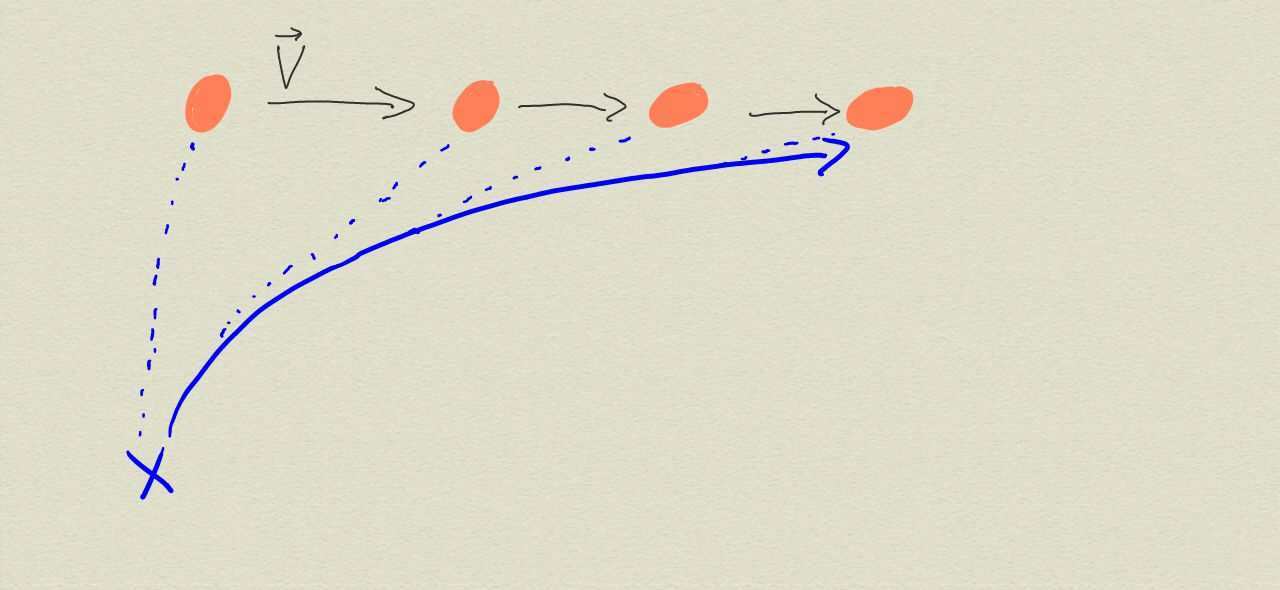
\includegraphics[width=7cm]{img/cap6/planning01}
  }
  \subfloat[Trayectoria rectilínea]{
    \label{fig:planning02}
    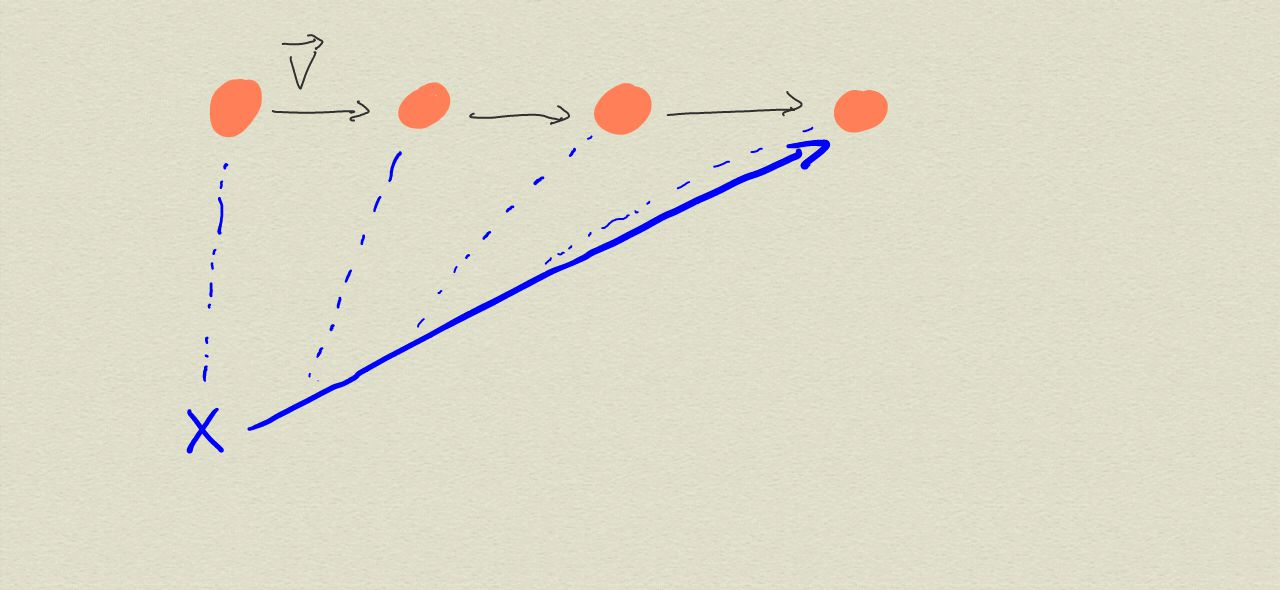
\includegraphics[width=7cm]{img/cap6/planning02}
  }
  \caption{Diferencia de trayectoria con/sin tener en cuenta la velocidad de la bola}
  \label{fig:planning}
\end{figure}

En la figura \ref{fig:planning01} se puede ver la típica trayectoria que toma un jugador que sólo conoce las posiciones instantáneas de la pelota. Es una trayectoria con forma de parábola. Según se acerca el jugador a la pelota, está se va moviendo y el robot siempre toma las decisiones con retraso. En cambio, si se conoce la posible posición final de la pelota -figura \ref{fig:planning02}- , se puede ir directamente a esta localización y utilizar el sistema de visión, simplemente para comprobar que la hipótesis es correcta y, al mismo tiempo, realizar pequeños ajustes.

\item Seguimiento de otros jugadores. El algoritmo se puede utilizar también para realizar el seguimiento de los otros robots que están en el campo. Esto puede ayudar enormemente en el cálculo de caminos para evitar a los jugadores con antelación.

\item Estado compartido de la pelota. Se pueden introducir observaciones de otros jugadores para intentar mejorar la percepción de la pelota, llegando incluso al punto de conocer la posición de la pelota sin ni siquiera verla.

\end{itemize}
